\documentclass[a4paper,12pt]{article}
\usepackage[indonesian]{babel}
\usepackage{graphicx}
\usepackage{multirow}
\usepackage{enumitem}
\usepackage{listings}
\usepackage{wrapfig}
\usepackage[T1]{fontenc}
\usepackage{inconsolata}
\usepackage{lipsum}
\usepackage{adjustbox}


\usepackage{color}
\usepackage[table]{xcolor}
\definecolor{mygreen}{rgb}{0,0.6,0}
\definecolor{mygray}{rgb}{0.5,0.5,0.5}
\definecolor{mymauve}{rgb}{0.58,0,0.82}
\lstset{%
    language=java,
    showstringspaces=false,          % Prevent tex replacing space to bracket in code
    frame=single,                    % Set frame around code
    backgroundcolor=\color{white},   % choose the background color
    basicstyle=\footnotesize,        % size of fonts used for the code
    breaklines=true,                 % automatic line breaking only at whitespace
    captionpos=b,                    % sets the caption-position to bottom
    commentstyle=\color{mygreen},    % comment style
    keywordstyle=\color{blue},       % keyword style
    stringstyle=\color{mymauve},     % string literal style
    numbers=left,
}

\graphicspath{ {./img/} }
\begin{document}
\title{ {\Large Laporan Praktikum}\\ Struktur Data\\{\Large Pertemuan 2}}

\author{Aldzikri Dwijayanto Prathama
    \\195410189
    \\Informatika}
\makeatletter
\begin{titlepage}
    \begin{center}
        {\huge \bfseries \@title}\\[14ex]
        
\includegraphics[scale=.8]{logo}\\[4ex]
        {\large \@author}\\[12ex]
        {\large \bfseries {SEKOLAH TINGGI MANAJEMEN INFORMATIKA DAN KOMPUTER
            AKAKOM YOGYAKARTA}}
    \end{center}


%{\large \@date}
\end{titlepage}
\makeatother
%\maketitle
\newpage
\tableofcontents
\newpage

\section{Tujuan}
mahasiswa dapat membuat suatu struktur \textit{record} (rekaman) dan \textit{array of record}
(rekaman dalam larik) untuk menyimpan data mengunakan bahasa java.
\section{Dasar Teori}
 
Pada percobaan terdahulu (modul 1) kita telah belajar bagaimana membuat media penyimpanan (variabel) menggunakan
tipe data \textit{primitive} baik itu tipe alphabetic, tipe data numeric maupun tipe data \textit{array}/larik.\\

Pada modul 2 ini kita akan lebih banyak belajar bagaimana membuat media penyimpanan berbasis \textit{record}
(rekaman). Record sering juga disebut Obyek/Simpul/List/Node/Senarai. Dalam pembuatannya, record didefinisikan sebagai
variabel bertipe data buatan (harus dideklarasikan menggunakan class).

\newpage

\section{Pembahasan}
\subsection{Praktik}
\subsubsection{Praktik 1}
\paragraph*{Struktur Penyimpanan yang Tidak Terstruktur\\}
\begin{lstlisting}
import java.util.Scanner;

public class inputDataViaKeyboard {
    public static void main(String[] args) {
        String nama;
        String alamat;
        int umur;
        char jekel; // jenis kelamin
        String hobi[] = new String[3];
        float ipk;
        Scanner masukan = new Scanner(System.in);
        int bacaTombol = 0;
        System.out.print("Silakan masukkan nama anda : ");
        nama = masukan.next();
        System.out.print("Silakan masukkan alamat anda : ");
        alamat = masukan.next();
        System.out.print("Silakan masukkan umur anda : ");
        umur = masukan.nextInt();
        System.out.print("Silakan masukkan Jenis Kelamin anda : ");
        try {
            bacaTombol = System.in.read();
        }catch (java.io.IOException e) {
        }
        jekel = (char) bacaTombol;
        System.out.println("Silakan masukkan hobi (maks 3) : ");
        System.out.print("hobi ke-0 : ");
        hobi[0] = masukan.next();
        System.out.print("hobi ke-1 : ");
        hobi[1] = masukan.next();
        System.out.print("hobi ke-2 : ");
        hobi[2] = masukan.next();
        System.out.print("Silakan masukkan IPK anda : ");
        ipk = masukan.nextFloat();
        System.out.println("Nama anda adalah " + nama);
        System.out.println("Nama alamat adalah " + alamat);
        System.out.println("Umur anda adalah " + umur);
        System.out.println("Jenis Kelamin anda adalah " + jekel);
        System.out.println("Hobi ke-0 anda adalah " + hobi[0]);
        System.out.println("Hobi ke-1 anda adalah " + hobi[1]);
        System.out.println("Hobi ke-2 anda adalah " + hobi[2]);
        System.out.println("IPK anda adalah " + ipk);
    }
}
\end{lstlisting}
Pada program di atas terdapat beberapa variabel, yang meskipun variabel tersebut terlihat seperti sebuah kesatuan
variabe yang saling berhubungan, namun sebenarnya variabel nama, alamat, umut, jekel, hobi[], dan ipk bukanlah suatu
kesatuan yang utuh.\\
Hal ini disebabkan karena masing-masing variabel tersebut dideklarasi secara terpisah menggunakan tipe datamasing-masing
sehingga tentu akan membentuk suatu struktur penyimpan yang terpisah pula sekalipun datanya adalahdata milik satu orang
(”AgungBP”; ”Jakarta”,28, ’L’,”musik”, ”mancing”, ”touring” ,3.5).\\
Jika program dijalankan, akan menghasilkan output seperti berikut:
\begin{center}
    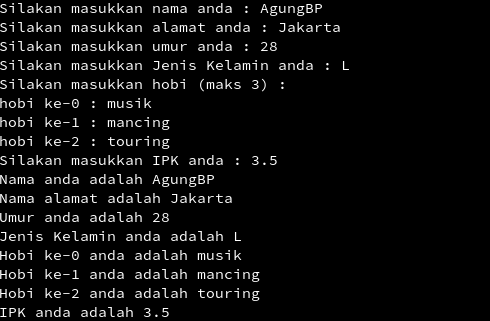
\includegraphics[scale=1]{prog12.png} 
\end{center}

\paragraph*{Struktur Penyimpanan yang Terstruktur\\}
\begin{lstlisting}
import java.util.Scanner;
class formatBiodata { // bagian deklarasi struktur record ----------------------------------
    String nama;
    String alamat;
    int umur;
    char jekel;
    String hobi[] = new String[3];
    float ipk;
}

public class strukturRekamanData {
    public static void main(String[] args) { // bagian deklarasi record --------------------------------------
        formatBiodata biodataMahasiswa = new formatBiodata();
        // bagian entri data melalui keyboard ---------------------------
        Scanner masukan = new Scanner(System.in);
        int bacaTombol = 0;
        System.out.print("Silakan masukkan nama anda : ");
        biodataMahasiswa.nama = masukan.next();
        System.out.print("Silakan masukkan alamat anda : ");
        biodataMahasiswa.alamat = masukan.next();
        System.out.print("Silakan masukkan umur anda : ");
        biodataMahasiswa.umur = masukan.nextInt();
        System.out.print("Silakan masukkan Jenis Kelamin anda : ");
        try {
            bacaTombol = System.in.read();
        } catch (java.io.IOException e) {
        }
        biodataMahasiswa.jekel = (char) bacaTombol;
        System.out.println("Silakan masukkan hobi (maks 3) : ");
        System.out.print("hobi ke-0 : ");
        biodataMahasiswa.hobi[0] = masukan.next();
        System.out.print("hobi ke-1 : ");
        biodataMahasiswa.hobi[1] = masukan.next();
        System.out.print("hobi ke-2 : ");
        biodataMahasiswa.hobi[2] = masukan.next();
        System.out.print("Silakan masukkan IPK anda : ");
        biodataMahasiswa.ipk = masukan.nextFloat();
        System.out.println("Nama anda adalah " + biodataMahasiswa.nama);
        System.out.println("Nama alamat adalah " + biodataMahasiswa.alamat);
        System.out.println("Umur anda adalah " + biodataMahasiswa.umur);
        System.out.println("Jenis Kelamin anda " + biodataMahasiswa.jekel);
        System.out.println("Hobi ke-0 anda " + biodataMahasiswa.hobi[0]);
        System.out.println("Hobi ke-1 anda " + biodataMahasiswa.hobi[1]);
        System.out.println("Hobi ke-2 anda " + biodataMahasiswa.hobi[2]);
    }
}
\end{lstlisting}
Dari program di atas, walaupun hasil eksekusinya sama dengan program sebelumnya, 
namun secara struktur kedua program tersebut sangat jauh berbeda. Pada program ini 
anda  dapat melihat bahwa ada sebuah variabel bernama  biodataMahasiswa yang 
berfungsi untuk menyatukan variabel yang lebih kecil yang berupa nama, alamat, umur, 
jekel, hobi [ ] dan ipk.\\ 
 
Jika kita  lihat pada bagian deklarasi, variabel biodataMahasiswa ini tidaklah 
dibentuk menggunakan tipe data primitif seperti string, char, int, dan lainnya, tetapi  
dideklarasikan dalam tipe data bernama formatBiodata. Tipe data formatBiodata ini 
tidaklah dikenal oleh Java karena memang bukanlah tipe bawaan dari java. Karena tipe 
data ini bukanlah bawaan java melainkan merupakan ciptaan programmer maka tipe 
data ini yang disebut dengan tipe data buatan. \\
 
Dalam pembuatannya, tipe data buatan dibentuk dengan melibatkan 
penggunaan kelas (class), sedangkan variabelnya sendiri yaitu biodataMahasiswa 
disebut sebagai obyek. (anda akan mempelajari class dan obyek lebih jauh dalam 
Pemrograman Berorientasi Obyek). Variabel atau obyek yang bernama 
biodataMahasiswa ini akan menjadi pembungkus atau wadah bagi variabel-variabel 
yang lebih kecil yaitu nama, alamat, umur, jekel, hobi[ ] dan ipk.\\
Dari tata cara penyebutannya, memang akhirnya penyebutan variabel nama, 
alamat, umur, jekel, dan juga ipk tidaklah menjadi sederhana karena penyebutannya 
harus senantiasa didahului dengan menyebut nama obyeknya terlebih dahulu baru 
kemudian disusul dengan tanda titik (.) dan dilanjutkan dengan penyebutan nama variabelnya\\
Sekalipun terlihat lebih rumit, dengan menggunakan struktur penyimpan yang 
telah dipaparkan di atas kita telah dapat memastikan bahwa data-data 
”AgungBP”,”Jakarta”, 28,’L’, ”musik”, ”mancing”, ”touring” 
3.5  yang tersimpan dalam variabel nama, alamat, umur, jekel, 
hobi[0], hobi[1], hobi[2], ipk adalah biodata milik seorang pribadi yang 
sama. Dengan demikian model penyimpan data tersebut sudah dapat diartikan 
merupakan model penyimpan data yang terstruktur.\\ 
Karena fungsinya yang dapat membungkus atau menyatukan beberapa variabel 
yang terpisah maka konsep penyimpanan data seperti ini juga dapat disebut dengan konsep penyimpanan data yang
terstruktur.\\
Jika program dijalankan akan menghasilkan keluaran berikut:
\begin{center}
    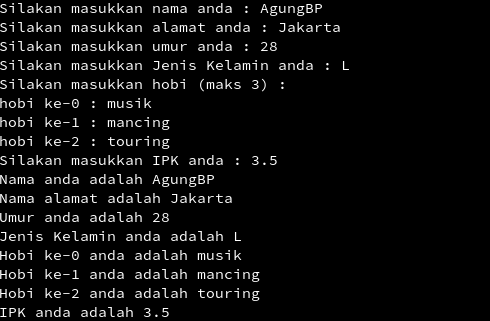
\includegraphics[scale=1]{prog12.png} 
\end{center}

\paragraph*{Struktur Penyimpanan Berbasis Array of Record (Rekaman dalam Larik)\\}
\begin{lstlisting}
import java.util.Scanner;

class formatBiodata { // bagian deklarasi struktur record ----------------------------------
    String nama;
    String alamat;
    int umur;
    char jekel;
    String hobi[] = new String[3];
    float ipk;
}

class strukturRekamanData2 {
    public static void main(String[] args) {
        int N = 5;
        // bagian deklarasi record berbasis LARIK -----------------------
        formatBiodata biodataMahasiswa[] = new formatBiodata[5];
        biodataMahasiswa[0] = new formatBiodata();
        biodataMahasiswa[1] = new formatBiodata();
        biodataMahasiswa[2] = new formatBiodata();
        biodataMahasiswa[3] = new formatBiodata();
        biodataMahasiswa[4] = new formatBiodata();
        // bagian entri data ke dalam struktur larik -----------------------
        Scanner masukan = new Scanner(System.in);
        int bacaTombol = 0;
        for (int i = 0; i <= N - 1; i++) {
            System.out.print("Silakan masukkan nama anda : ");
            biodataMahasiswa[i].nama = masukan.next();
            System.out.print("Silakan masukkan alamat anda : ");
            biodataMahasiswa[i].alamat = masukan.next();
            System.out.print("Silakan masukkan umur anda : ");
            biodataMahasiswa[i].umur = masukan.nextInt();
            System.out.print("Silakan masukkan Jenis Kelamin anda : ");
            try {
                bacaTombol = System.in.read();
            } catch (java.io.IOException e) {
            }
            biodataMahasiswa[i].jekel = (char) bacaTombol;
            System.out.println("Silakan masukkan hobi (maks 3) : ");
            System.out.print("hobi ke-0 : ");
            biodataMahasiswa[i].hobi[0] = masukan.next();
            System.out.print("hobi ke-1 : ");
            biodataMahasiswa[i].hobi[1] = masukan.next();
            System.out.print("hobi ke-2 : ");
            biodataMahasiswa[i].hobi[2] = masukan.next();
            System.out.print("Silakan masukkan IPK anda : ");
            biodataMahasiswa[i].ipk = masukan.nextFloat();
            System.out.println("");
        }
        // bagian menampilkan isi struktur Larik -------------------------
        System.out.println("-------------------------------------------");
        System.out.println("NAMA ALAMAT UMUR JEKEL HOBI1 HOBI2 HOBI3 IPK");
        System.out.println("-------------------------------------------");
        for (int i = 0; i <= N - 1; i++) {
            System.out.print(biodataMahasiswa[i].nama + "  ");
            System.out.print(biodataMahasiswa[i].alamat + "  ");
            System.out.print(biodataMahasiswa[i].umur + "  ");
            System.out.print(biodataMahasiswa[i].jekel + "  ");
            System.out.print(biodataMahasiswa[i].hobi[0] + "  ");
            System.out.print(biodataMahasiswa[i].hobi[1] + "  ");
            System.out.print(biodataMahasiswa[i].hobi[2] + "  ");
            System.out.println(biodataMahasiswa[i].ipk);
        }
        System.out.println("-------------------------------------------");
    }
}
\end{lstlisting}
Pada program ini sedikit berbeda dengan program sebelumnya, karena variabel menggunakan array , maka penyebutan nama
obyek yang mendahului penyebutan variabel nama, alamat, umur, jenis kelamin, dan ipk harus diikuti dengan tanda
kurung[], karena variabel berjenis array.\\
Program ini dibuat sebuah struktur penyimpanan array yang berorientasi pada record. Program dapat menampung 5 orang
data mahasiswa.\\
Jika program dijalankan maka akan menghasilkan output seperti berikut ini:
\begin{center}
    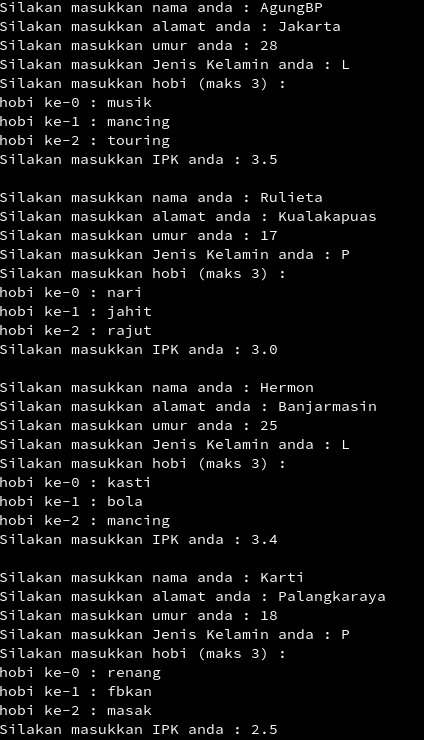
\includegraphics[scale=1]{prog34a.png} 
    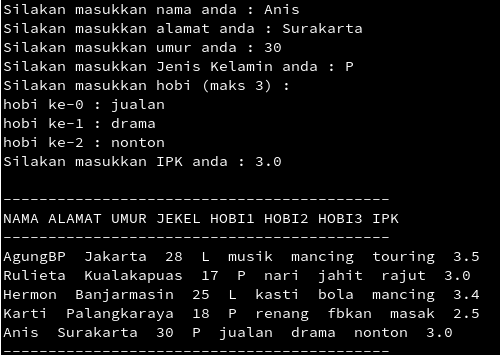
\includegraphics[scale=1]{prog34b.png} 
\end{center}

\paragraph*{Pembuatan Program Secara Modular (Fungsi)\\}
\begin{lstlisting}
import java.util.Scanner;

class formatBiodata2 { // bagian deklarasi struktur record ---------------------------------
    String nama;
    String alamat;
    int umur;
    char jekel;
    String hobi[] = new String[3];
    float ipk;
}

class pertemuan3 {
    public static int N = 5;
    // --------------------------------------------------
    // --- Fungsi untuk mengentri data ke dalam Larik ---
    // --------------------------------------------------
    public static void ngentriData(formatBiodata biodataMahasiswa[]) {
        // bagian entri data ke dalam struktur larik ----------------
        Scanner masukan = new Scanner(System.in);
        int bacaTombol = 0;
        for (int i = 0; i <= N - 1; i++) {
            System.out.print("Silakan masukkan nama anda : ");
            biodataMahasiswa[i].nama = masukan.next();
            System.out.print("Silakan masukkan alamat anda : ");
            biodataMahasiswa[i].alamat = masukan.next();
            System.out.print("Silakan masukkan umur anda : ");
            biodataMahasiswa[i].umur = masukan.nextInt();
            System.out.print("Silakan masukkan Jenis Kelamin anda : ");
            try {
                bacaTombol = System.in.read();
            } catch (java.io.IOException e) {
            }
            biodataMahasiswa[i].jekel = (char) bacaTombol;
            System.out.println("Silakan masukkan hobi (maks 3) : ");
            System.out.print("hobi ke-0 : ");
            biodataMahasiswa[i].hobi[0] = masukan.next();
            System.out.print("hobi ke-1 : ");
            biodataMahasiswa[i].hobi[1] = masukan.next();
            System.out.print("hobi ke-2 : ");
            biodataMahasiswa[i].hobi[2] = masukan.next();
            System.out.print("Silakan masukkan IPK anda : ");
            biodataMahasiswa[i].ipk = masukan.nextFloat();
            System.out.println();
        }
    }

    // --------------------------------------------------
    // --- Fungsi untuk menampilkan data ---
    // --------------------------------------------------
    public static void tampilkanData(formatBiodata biodataMahasiswa[]) {
        // bagian menampilkan isi struktur Larik --------------------------
        System.out.println("---------------------------------------------");
        System.out.println("NAMA ALAMAT UMUR  JEKEL HOBI1 HOBI2 HOBI3 IPK");
        System.out.println("---------------------------------------------");
        for (int i = 0; i <= N - 1; i++) {
            System.out.print(biodataMahasiswa[i].nama + "  ");
            System.out.print(biodataMahasiswa[i].alamat + "  ");
            System.out.print(biodataMahasiswa[i].umur + "  ");
            System.out.print(biodataMahasiswa[i].jekel + "  ");
            System.out.print(biodataMahasiswa[i].hobi[0] + "  ");
            System.out.print(biodataMahasiswa[i].hobi[1] + "  ");
            System.out.print(biodataMahasiswa[i].hobi[2] + "  ");
            System.out.println(biodataMahasiswa[i].ipk);
        }
        System.out.println("---------------------------------------------");
    }

    // --------------------------------------------------
    // --- Program Utama ---
    // --------------------------------------------------
    public static void main(String[] args) { // bagian deklarasi record berbasis LARIK -----------------------
        formatBiodata biodataMahasiswa[] = new formatBiodata[10];
        biodataMahasiswa[0] = new formatBiodata();
        biodataMahasiswa[1] = new formatBiodata();
        biodataMahasiswa[2] = new formatBiodata();
        biodataMahasiswa[3] = new formatBiodata();
        biodataMahasiswa[4] = new formatBiodata();
        ngentriData(biodataMahasiswa);
        tampilkanData(biodataMahasiswa);
    }
}
\end{lstlisting}
Program diatas merupakan program sebelumnya yang dimodifikasi sehingga lebih modular, jika dicermati, program
sebelumnya mempunyai 3 bagian besar. Yang pertama deklarasi, lalu entri data, kemudian penampilan data. Oleh karena itu
pada program ini code ditulis secara lebih modular berdasarkan ketiga bagian tadi.\\
Jika program ini dijalankan akan menghasilkan output berikut:\\
\begin{center}
    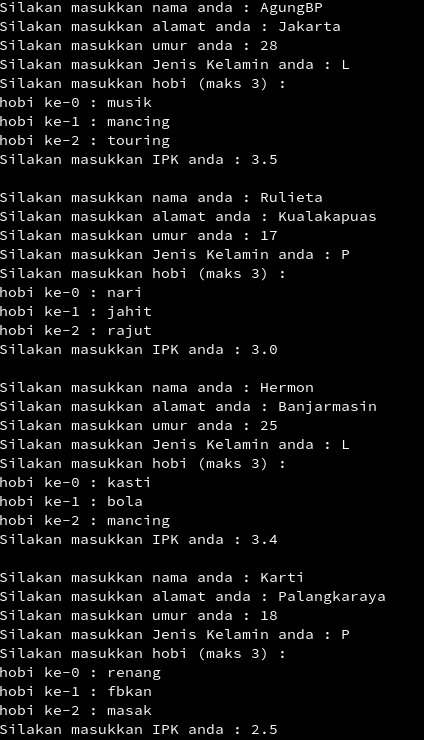
\includegraphics[scale=1]{prog34a.png} 
    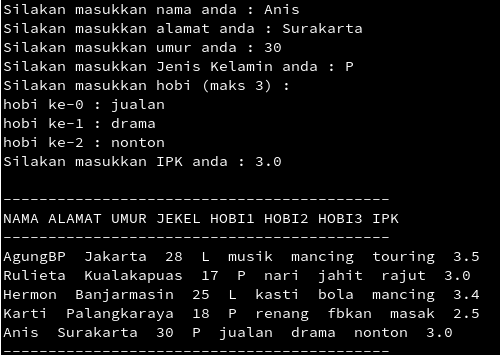
\includegraphics[scale=1]{prog34b.png} 
\end{center}

\subsubsection{Praktik 2}
\begin{lstlisting}
import java.util.Scanner;

class formatBiodata { // bagian deklarasi struktur record ---------------------------------
    String nama;
    String alamat;
    int umur;
    char jekel;
    String hobi[] = new String[3];
    float ipk;
}

class Praktik2 {
    public static int N = 10;
    // --------------------------------------------------
    // --- Fungsi untuk mengentri data ke dalam Larik ---
    // --------------------------------------------------
    public static void ngentriData(formatBiodata biodataMahasiswa[]) {
        // bagian entri data ke dalam struktur larik ----------------
        Scanner masukan = new Scanner(System.in);
        int bacaTombol = 0;
        for (int i = 0; i <= N - 1; i++) {
            System.out.print("Silakan masukkan nama anda : ");
            biodataMahasiswa[i].nama = masukan.next();
            System.out.print("Silakan masukkan alamat anda : ");
            biodataMahasiswa[i].alamat = masukan.next();
            System.out.print("Silakan masukkan umur anda : ");
            biodataMahasiswa[i].umur = masukan.nextInt();
            System.out.print("Silakan masukkan Jenis Kelamin anda : ");
            try {
                bacaTombol = System.in.read();
            } catch (java.io.IOException e) {
            }
            biodataMahasiswa[i].jekel = (char) bacaTombol;
            System.out.println("Silakan masukkan hobi (maks 3) : ");
            System.out.print("hobi ke-0 : ");
            biodataMahasiswa[i].hobi[0] = masukan.next();
            System.out.print("hobi ke-1 : ");
            biodataMahasiswa[i].hobi[1] = masukan.next();
            System.out.print("hobi ke-2 : ");
            biodataMahasiswa[i].hobi[2] = masukan.next();
            System.out.print("Silakan masukkan IPK anda : ");
            biodataMahasiswa[i].ipk = masukan.nextFloat();
            System.out.println();
        }
    }

    // --------------------------------------------------
    // --- Fungsi untuk menampilkan data ---
    // --------------------------------------------------
    public static void tampilkanData(formatBiodata biodataMahasiswa[]) {
        // bagian menampilkan isi struktur Larik --------------------------
        System.out.println("---------------------------------------------");
        System.out.println("NAMA ALAMAT UMUR  JEKEL HOBI1 HOBI2 HOBI3 IPK");
        System.out.println("---------------------------------------------");
        for (int i = 0; i <= N - 1; i++) {
            System.out.print(biodataMahasiswa[i].nama + "  ");
            System.out.print(biodataMahasiswa[i].alamat + "  ");
            System.out.print(biodataMahasiswa[i].umur + "  ");
            System.out.print(biodataMahasiswa[i].jekel + "  ");
            System.out.print(biodataMahasiswa[i].hobi[0] + "  ");
            System.out.print(biodataMahasiswa[i].hobi[1] + "  ");
            System.out.print(biodataMahasiswa[i].hobi[2] + "  ");
            System.out.println(biodataMahasiswa[i].ipk);
        }
        System.out.println("---------------------------------------------");
    }

    // --------------------------------------------------
    // --- Program Utama ---
    // --------------------------------------------------
    public static void main(String[] args) { // bagian deklarasi record berbasis LARIK -----------------------
        formatBiodata biodataMahasiswa[] = new formatBiodata[10];
        biodataMahasiswa[0] = new formatBiodata();
        biodataMahasiswa[1] = new formatBiodata();
        biodataMahasiswa[2] = new formatBiodata();
        biodataMahasiswa[3] = new formatBiodata();
        biodataMahasiswa[4] = new formatBiodata();
        biodataMahasiswa[5] = new formatBiodata();
        biodataMahasiswa[6] = new formatBiodata();
        biodataMahasiswa[7] = new formatBiodata();
        biodataMahasiswa[8] = new formatBiodata();
        biodataMahasiswa[9] = new formatBiodata();
        ngentriData(biodataMahasiswa);
        tampilkanData(biodataMahasiswa);
    }
}
\end{lstlisting}
Program pada praktik 2 ini merupakan hasil dari modifikasi dari program sebelumnya, sehingga program dapat
menyimpan data untuk 10 orang mahasiswa.\\
Agar program mampu memuat 10 data mahasiswa, ada beberapa bagian yang dimodifikasi.\\
Pertama yaitu variabel int N, yang tadinya memiliki nilai 5, diubah menjadi 10.\\
Kedua pada bagian pendeklarasian variabel array, yang tadinya hanya sampai array ke 4, ditambahkan lagi sampai array
ke 9.\\
Jika program dijalankan, maka akan memiliki output seperti berikut:
\begin{center}
    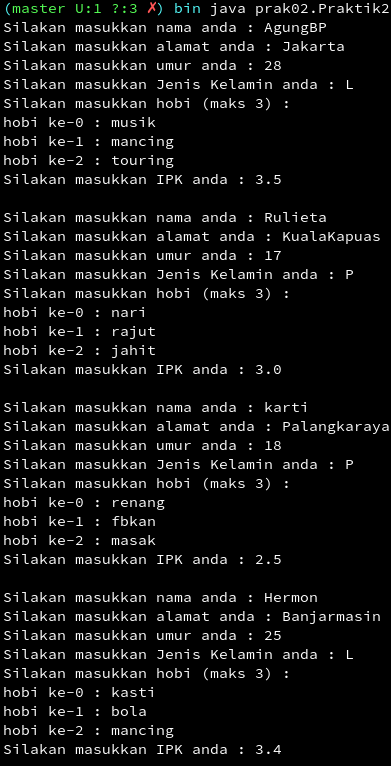
\includegraphics[scale=1]{out-prak2-1.png} 
    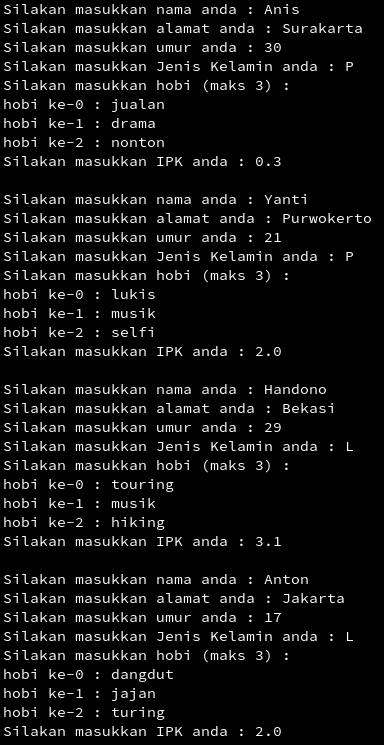
\includegraphics[scale=1]{out-prak2-2.png} 
    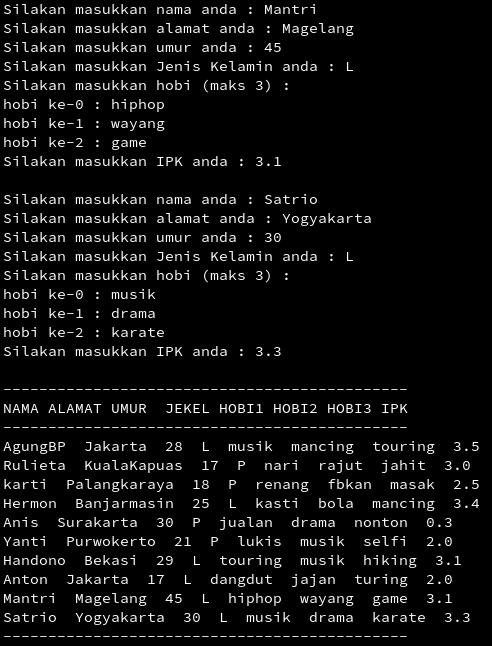
\includegraphics[scale=1]{out-prak2-3.png} 
\end{center}

\subsection{Latihan}

\subsection{Tugas}

\newpage

\section{Kesimpulan}
Setelah praktik mahasiswa dapat menggunakan berbagai tipe data untuk menyimpan data baik alphabetic, alphanumeric,
maupun boolean.
\end{document}
